\documentclass{article}

\usepackage[utf8]{inputenc}
\usepackage[T1]{fontenc}
\usepackage[catalan]{babel}
\usepackage{amsmath, amssymb, amsthm}
\usepackage{graphicx}
\usepackage[colorlinks,linkcolor=blue,citecolor=blue,urlcolor=blue]{hyperref}

\renewcommand{\baselinestretch}{1.5}

\title{Pràctica 3: Interpolació i Integració Numèrica}
\author{Cristina Rosell Blanco: 1457235  \\ Oriol Ventosa Altimira: 1457285}
\date{11 de març de 2018}
\begin{document}
	\maketitle
	
	\newpage

	\section{Problema 1}
	
	\paragraph{a:} 
	Primer observem com és la funció que volem aproximar:
	
	\begin{center}
		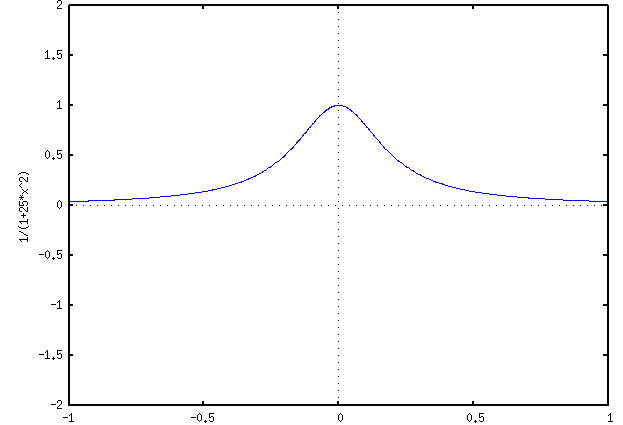
\includegraphics[width=8cm]{funcio.png}
	\end{center}
	
	Començarem analitzem com evoluciona l'error màxim en els nodes equidistants.
	
	Executant el programa en 4, 8, 16, 32 i 64 nodes obtenim que l'error va creixen, desde 0.4383 amb 8 nodes fins a 982148169.3852 amb 64 nodes.
	
	Ens dibuixem les diferents aproximacions en un gràfic:
	
	\begin{center}
		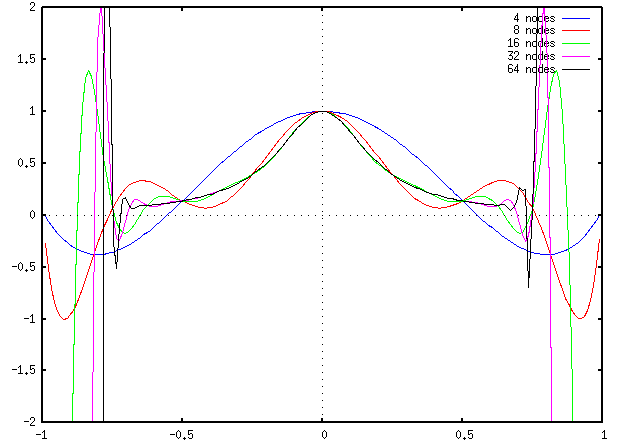
\includegraphics[width=12cm]{equi.png}
	\end{center}
	
	Observem que en totes les aproximacions el interval [-0.5,0.5] la funció s'aproxima prou bé, però a mesura que ens acostem als extrems de la funció el error es dispara, cada vegada més a mesura que augmentem els nodes.
	
	Ara analitzem el error amb els nodes de Chebyshev, en aquest cas amb 4 nodes el error màxim és 0.4018, va descreixent fins al 32 nodes amb un error de 0.00139 i quan calculem l'aproximació amb 64 nodes l'error màxim es dispara a 4.5780.
	
	Ara dibuixem les diferents aproximacions de nou:
	
	\begin{center}
		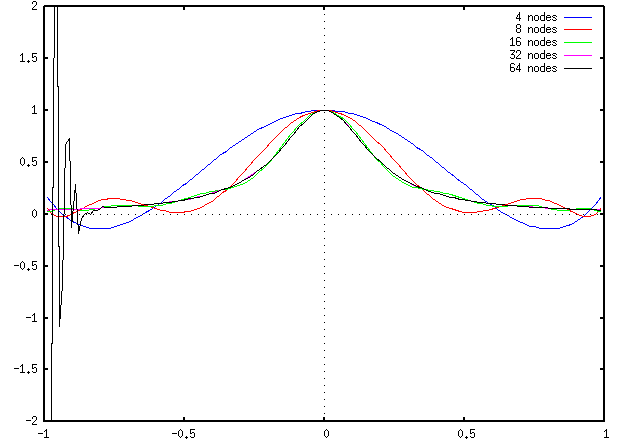
\includegraphics[width=12cm]{cheb.png}
	\end{center}
	
	Observem que a mesura que els nodes augmenten l'error disminueix, i a 64 el error a l'extrem esquerra és molt gran, però veiem que un cop ens allunyem de l'extrem l'error és molt petit.
	
	\paragraph{b:} La raó per la qual els errors entre els dos mètodes per fer particions són tant diferents és el que s'anomena fenòmen de Runge.
	
	Aquest fenòmen explica que amb certs tipus de funcions, com  la que hem aproximat, quan és crea el polinomi interpolador a partir de particions equidistants l'error a mesura que augmenten els nodes tendeix a infinit als extrems.
	
	Per això quan hem utilitzat els nodes de Chebyshev l'error ha disminuit.
	
	\newpage
	
	\section{Problema 2}
	
	Considerant que la funció és continua i monotona, l'arrel es trobarà entre els dos nodes que tenen un canvi de signe.
	
	De manera que si utilitzem els polinomis interpoladors trobats en el apartat a i b, agafar només valors positius o negatius, el que estariem fent seria extrapolar el valor l'arrel amb el polinomi interpolador, ja que haurem agafat un interval de nodes que no embarca l'arrel.
	
	En canvi, en el apartat c l'arrel si que es trobarà en el interval dels nodes, de manera que el resultat hauria de ser més precís amb el polinomi interpolador d'aquest apartat.
	
	\textbf{Apartat a:}
	
	Grau 1 dona: 2.404728613882804
	
	Grau 3 dona: 2.404822718113948
	
	Grau 5 dona: 2.40482529478546
	
	\textbf{Apartat b:}
	
	Grau 1 dona: 2.400077241947102
	
	Grau 3 dona: 2.404149375353532
	
	Grau 5 dona: 2.404216734868259
	
	\textbf{Apartat c:}
	
	Grau 1 dona: 2.404927513002775
	
	Grau 3 dona: 2.404824021911155
	
	Grau 5 dona: 2.404825653043717
	
	Avaluant la funció de Bessel amb les aproximacions de 5 particions obtenim que el apartat c aproxima l'arrel amb un error de $5x10^{-8}$, el apartat b amb un error de $2x10^{-7}$ i l'apartat a amb un error de $3x10^{-4}$.
	
	\newpage
	
	\section{Problema 3}
	La integral $$\int \limits_{0}^{1} \frac{dx}{1+x^2}$$ amb el mètode dels trapezis ens dóna de resultat 0.7827941176470589, en canvi, amb el mètode de Simpson ens dóna 0.7853921568627452. Veiem que el resultat que obtenim amb trapezis té només dues xifres significatives, mentre que amb Simpson en té cinc.
		
	L'error amb el mètode dels trapezis ve donat per $\frac{f''(\xi)}{12}h^3$. \\ Calculem la segona derivada: $f''(x)=\frac{6x^2-2}{(1+x^2)^3}$, observem que el màxim es troba en x=0, així doncs $|f''(0)|=2$. Per tant, l'error en valor absolut és $\frac{f''(\xi)}{12}h^3 = \frac{2}{12\cdot4^3} = \frac{1}{384} \textless 2'61\cdot10^{-3} $
		
	L'error amb el mètode de Simpson és $\frac{f^{4)}(\xi)}{90}h^5$. \\ Calculem la quarta derivada: $f^{4)}(x)=\frac{24(5x^4-10x^2+1)}{(1+x^2)^5}$, observem que el màxim es troba en x=0 també, així doncs $|f^{4)}(0)|=24$. Per tant, l'error en valor absolut és $\frac{f^{4)}(\xi)}{90}h^5 = \frac{24}{90\cdot4^5} = \frac{1}{3840} \textless 2'61\cdot10^{-4} $
		
		
	(cal revisar errors, tenia algo mal fet i no sé si ja està bé)
	
	\newpage	
		
	\section{Problema 4}
	Volem resoldre la integral $$\int \limits_{1}^{5} \frac{e^x}{x} dx$$
	a partir del mètode dels trapezis. Si dividim l'interval [1,5] en més o menys parts iguals, obtenim més precisió o menys, aquí veiem els resultats:
		
	\begin{figure}[h!]
		\begin{center}
			\begin{tabular}{|c|c|}
				\hline
				n & resultat \\ \hline
				4 & 40.23970135663446 \\ \hline
				8 & 38.7829281563148 \\ \hline
				16 & 38.41371136353941 \\ \hline
				32 & 38.32106916233212 \\ \hline
				64 & 38.2978869041288 \\ \hline
			\end{tabular}
		\end{center}
	\end{figure}
		
	Per calcular la cota d'error de la regla composta del trapezi utilitzarem la formula:
	
	$$-\frac{(b-a)f^{(2)}(\mu)}{12}h^2$$
	
	Volem trobar una cota per la segona derivada de $\frac{e^x}{x}$, que és $\frac{e^x(x^2-2x+2)}{x^3}$. 
	
	Mirant el gràfic de la derivada observem que el màxim es troba a x=5. Per tant
	$$f^{(2)}(x)\leq f^{(2)}(5)=43.93<44$$
	
	També tenim que $h=(b-a)/n=4/n$ on N és el nombre de particions.
	
	$$n=4\implies\frac{4*44}{12}=14.67$$
	
	que això implica que no té cap xifra significativa. Ara ho fem per la resta de particions
	
	\vspace{6cm}
	
	\begin{figure}[h!]
		\begin{center}
			\begin{tabular}{|c|c|}
				\hline
				n & Error \\ \hline
				4 & 14.67 \\ \hline
				8 & 3.67 \\ \hline
				16 & 0.9167 \\ \hline
				32 & 0.2292 \\ \hline
				64 & 0.0573 \\ \hline
			\end{tabular}
		\end{center}
	\end{figure}
	
	I d'aquí deduïm que només podem esperar obtenir un decimal significatiu a partir de 64 particions.
	
	\newpage
		
	\section{Problema 5}
	
	Mitjançant la fórmula de Simpson, aconseguim acotar la integral amb una precisió de $10^{-2}$ utilitzant només dues particions, i aconseguim el resultat de 0.3858346021654338.
	
	\newpage
	
	\section{Problema 6}
	
	Sens presenta una funció de la velocitat respecte el temps de manera discreta. Per aproximar quina serà la longitud de la pista aplicarem la formula de Simpson composta amb els segons com a nodes i la velocitat com la imatge d'aquests nodes.
	
	Un cop fet obtenim que l'aproximació de la longitud de la pista és 2904.4.
	
	Si volguessim millorar aquesta aproximació el que hauriem de fer és trobar nous nodes aproximant la funció amb mètodes interpoladors.
	
	Per exemple, hem buscat el polinomi interpolador amb els nodes donats i l'hem aplicat en els segons de la forma $3+6n$, i ,afegint aquests nodes als antics i aplicant Simpson de nou, l'aproximació de la longitud de la pista dona: 2497.1.
		
\end{document}
